\section{Experiment 1: simulated data from multivariate normal distribution}

	In the first simulation experiment, we focused on an ideal setting where data came from a known multivariate normal 
	distribution and imputation was required to estimate the means, variances, and covariances of six items with 
	missing values.
	We investigated the relative performance of the methods described above across a set of conditions defined by two 
	experimental factors: the number of columns in the dataset, $p$, taking values 50 or 500; 
	and the proportion of missing cases on each variable, $pm$, taking values 0.1 or 0.3.
	Table \ref{tab:condExp1} summarizes the four resulting crossed conditions.
	Data with sample size $n=200$ were independently generated $S = 1,000$ times for each condition.
	For each $s$th replicate, missing values were imposed on six target items, and then all missing data treatment methods described above
	were used to obtain estimates of the item means, variances, and covariances.

\begin{table}
\tbl{Summary of conditions for Experiment 1.}
	{
	\begin{tabular}{l c c c c } 
		\toprule
		condition & label & n & p & pm \\
		\midrule
		1 & low-dim-low-pm   & 200 & 50  & 0.1 \\
		2 & high-dim-low-pm  & 200 & 500 & 0.1 \\
		3 & low-dim-high-pm  & 200 & 50  & 0.3 \\
		4 & high-dim-high-pm & 200 & 500 & 0.3 \\
		\bottomrule
	\end{tabular}
	}
\label{tab:condExp1}
\end{table}

%\FloatBarrier

\subsection{Simulation study procedure}

\subsubsection{Data generation}
	At every replication, a data matrix $\bm{Z}_{n \times p}$ was generated according to a multivariate normal model centered around a vector of fives and covariance matrix $\bm{\Sigma}_0$. The diagonal elements of $\bm{\Sigma}_0$ (variances) were equal to 1, and the off-diagonal elements were used to define three blocks of variables. 
	The first five variables were highly correlated among themselves ($\rho = 0.6$);
	variables 6 to 10 were weakly correlated with variables in block 1 and among themselves ($\rho = 0.3$), 
	and all the remaining $p-10$ variables were uncorrelated.

\subsubsection{Missing data imposition} \label{sub_missing}

	Missing values were imposed on six items in $\bm{Z}$: three variables in the block of
	highly correlated variables ($\bm{z}_j$ with $j = 1,2,3$), and three in the block of lowly correlated variables ($\bm{z}_j$ 
	with $j = 6,7,8$).
	Item nonresponse was imposed by sampling from a Bernoulli distribution with individual probabilities of nonresponse 
	defined by 
%
	\begin{equation} \label{eqn:rm}
		p_{miss} = p(z_{i,j} = miss | \tilde{\bm{Z}}) = \frac{ exp(\gamma_0 + \tilde{\bm{z}}_{i}\bm{\gamma}) }
								{ 1 + exp(\gamma_0 + \tilde{\bm{z}}_{i}\bm{\gamma}) }
	\end{equation}
%
	where $z_{i,j}$ is the $i$th subject's response on the $j$th target of missing data imposition, 
	$\tilde{\bm{z}}_{i}$ is a vector of responses to the set of missing data predictors for the $i$th individual, $\gamma_0$ is an intercept parameter, and $\bm{\gamma}$ is a vector of slope parameters.
	$\tilde{\bm{Z}}$ was specified to include two fully observed variables from the strongly correlated set and two 
	from the weakly correlated set ($\bm{z}_r$ with $r = 4,5,9,10$).
	The probability of nonresponse to a variable never depended on the variable itself. Therefore, by using all columns of $\bm{Z}_{-j,obs}$ as predictors in the MI procedures, the elements of $\tilde{\bm{Z}}$ 
	act as predictors in the imputation models, and the MAR assumption is satisfied.
	All slopes in $\bm{\gamma}$ were fixed to 1, while the value of $\gamma_0$ was chosen with an optimization 
	algorithm that minimized the difference between the actual and desired proportion of missing values.

\subsubsection{Imputation}
	
	Missing values were treated with all methods described in Section 2.
	To evaluate convergence of the imputation models, we ran ten replications of the high-dim-high-pm condition and checked trace plots of the means of the imputed values.
	These checks suggested that the imputation algorithms converged within 50 iterations. The only exception was blasso, which required approximately 2,000 iterations for convergence.

	The ridge penalty used in the bridge algorithm was fixed across iterations.
	We chose the value of the penalty term by means of a cross-validation procedure, wherein penalty values of $10^{-1}, 10^{-2}, ..., 10^{-8}$ were used to impute data with bridge. We then selected the value that resulted in the smallest average fraction of missing information
	\citep[FMI;][eq. 3.1.10]{rubin:1987} across the analysis model parameters. Both IURR and DURR could have been implemented with a variety of penalties (e.g., lasso, \citealp{tibshirani:1996}; elastic net, \citealp{zouHastie:2005}; adaptive lasso, \citealp{zou:2006}).
	In this study, we used lasso as it is computationally efficient, 
	and it performed well for imputation in \cite{zhaoLong:2016} and \cite{dengEtAl:2016}.
	A 10-fold cross-validation procedure was used at every iteration of DURR and IURR to choose the penalty parameter.

	To maintain consistency with previous research, we specified the blasso hyper-parameters in equations 
	\eqref{eqn:sigprior}, \eqref{eqn:tauprior}, and \eqref{eqn:rhoprior} as in \cite{zhaoLong:2016}: 
	$(a,b)=(0.1, 0.1)$, $(r,s)=(0.01, 0.01)$, and $(g,h)=(1,1)$.
	In the MI-PCA algorithm, we extracted enough components to explain 50\% of the total variance in the data.
	For the single random forest imputations, we used the \emph{missForest} R package 
	\citep{missForest} which implements Algorithm 1 from \cite{stekhovenBuhlmann:2011}.
	When evaluating convergence, we found that the stopping criterion for the missFor algorithm was usually met within the first 10 iterations, and we fixed the maximum number of iterations to 20.
	\cite{stekhovenBuhlmann:2011} recommended growing 100 trees per forest; therefore, we used this value in our study.

\subsubsection{Analysis}
	The substantive model of interest in Experiment 1 was a saturated model that estimated means,
	variances, and covariances of the six variables with missing values.
	Therefore, our analysis model estimated six means, six variances, and 15 covariances.

\subsection{Comparison criteria} \label{criteria}

	We compared the different missing data treatments in terms of bias and confidence interval coverage.

	\subsubsection{Bias}

	For a given parameter of interest $\theta$ (e.g., mean of item 1, variance of item 2), we used the 
	percent relative bias (PRB) to quantify the estimation bias introduced by the imputation procedure:
%
	\begin{equation} \label{eqn:prb}
		\textit{PRB} = \frac{\bar{\hat{\theta}} - \dot{\theta}}{\dot{\theta}} \times 100
	\end{equation}
%
	where $\dot{\theta}$ is the true value of the focal parameter defined as 
	$\sum_{s=1}^{S} \hat{\theta}_{s}^{GS}/S$
	, with
	$\hat{\theta}_{s}^{GS}$ 
	being the Gold Standard parameter estimate for the $s$th repetition. 
	The averaged focal parameter estimate under a given missing data treatment was computed as 
	$\bar{\hat{\theta}} = \sum_{s=1}^{S} \hat{\theta}_{s}/S$,
	with
	$\hat{\theta}_{s}$ being the estimate obtained from the treated incomplete data in the 
	$s$th repetition.
	Following \cite{muthenEtAl:1987}, we considered $|\text{PRB}| > 10$ as indicative of problematic 
	estimation bias.

	\subsubsection{Confidence intervals coverage}
	
	To assess the performance in hypothesis testing and interval estimation, we evaluated the confidence interval coverage (CIC) of the true parameter value:
%
	\begin{equation} \label{eqn:cic}
		\textit{CIC} =  \frac{ \sum_{s=1}^{S} I(\dot{\theta} \in \widehat{\textit{CI}}_s ) }{S}
	\end{equation}
%
	where $\widehat{\textit{CI}}_s$ is the confidence interval of the parameter estimate $\hat{\theta}_{s}$ in a given repetition, 
	and $I(.)$ is the indicator function that returns 1 if the argument is true and 0 otherwise.
	
	CICs below 0.9 are usually considered problematic for 95\% CIs \cite[p. 52]{vanBuuren:2018} 
	as they imply inflated Type I error rates.
	High CICs (e.g., 0.99) indicate CIs that are too wide, implying inflated Type II error rates.
	Therefore, we considered CIs to show severe under-coverage (over-coverage) if CIC $< 0.9$ (CIC $> 0.99$). From a testing perspective, a CIC can be considered as significantly different from the 
	nominal coverage rate if the magnitude of its difference from the nominal coverage probability, $p_0$, is more than two times the standard error of $p_0$, $\textit{SE}(p_0) = \sqrt{p (1-p)/S}$ \citep{burtonEtAl:2006}.
	Therefore, we considered 95\% CI coverages outside the interval $[0.94, 0.96]$ to be significantly different from the nominal coverage rate.

\subsection{Results}
	
	We computed both PRB and CIC for each of the 27 parameters in the analysis model (six means, six variances,
	and 15 covariances).
	To summarize the results, we focus on the typical and extreme values of these measures.
	In Figures \ref{fig:exp1bias} and \ref{fig:exp1cir}, we report the average, minimum, and maximum absolute PRB 
	and CIC for each missing data treatment method and each parameter type.
	In the supplementary material, we include figures reporting the raw PRB and CIC for every parameter estimate.

	\subsubsection{Means} 
	The largest $|\text{PRB}|$ for the means was below 10 for all 
	imputation methods. Only CC produced problematic degrees of bias.
	However, looking at the relative performances, IURR and MI-PCA resulted in smaller biases than all other methods 
	(except MI-OP).
	In terms of CIC, only bridge and MI-PCA showed consistently strong performance. Neither method demonstrated any extreme under-/over-coverage (i.e., CIC $\notin$ [0.9, 0.99]), and MI-PCA showed nonsignificant deviations from nominal coverage for 
	almost all estimates. DURR, IURR, and blasso demonstrated reasonable coverages when $pm$ was low, but tended to under-cover to problematic degrees when $pm$ was high.
	The tree-based methods and CC performed most poorly. These methods led to CICs significantly different from nominal coverage rates
	in all conditions and demonstrated extreme under-coverage in many conditions.

	\subsubsection{Variances} 
	IURR, blasso, and the tree-based MI methods resulted in low
	biases (i.e., $|\text{PRB}|< 10$) across all conditions.
	For blasso, these low biases were paired with low deviations from nominal coverage rates. IURR only demonstrated problematic CICs for the high-dim-high-pm
	condition where it produced extreme under-coverage. MI-CART and MI-RF only produced reasonable coverage rates when $pm$ was low. MI-PCA showed acceptable biases and reasonable coverage rates in all but the high-dim-high-pm condition where it showed large biases and extreme under-coverage. DURR showed poor performance with regard to the item variances. Although DURR produced acceptable levels of bias in all but the high-dim-high-pm condition, it produced extreme CI under-coverage in all but the low-dim-low-pm condition. Bridge, missFor, and CC performed poorly in nearly all conditions. These methods tended to demonstrate substantial biases and extreme under-coverage. Although bridge produced reasonable CICs with low $pm$, the extreme biases it produced negate any benefits of good coverage properties.

	\subsubsection{Covariances}
	
	MI-PCA was the only method that showed consistently strong performance when estimating covariances. MI-PCA showed negligible bias and minimal deviations from nominal coverage in all conditions.
	The MI-PCA never produced extreme under-/over-coverage, and when the CIC was significantly different from the nominal rate, the CIs showed mild \emph{over}-coverage (i.e., CICs greater than 0.96 but smaller than 0.99). After MI-PCA, IURR demonstrated the second strongest performance, with negligible bias and acceptable coverage in all but the high-dim-low-pm 
	condition. In the high-dim-high-pm condition, IURR produced large biases and extreme under-coverage.
	
	Bridge displayed low bias and acceptable coverage in the low dimensional conditions (columns 1 and 3 of Figures \ref{fig:exp1bias} and \ref{fig:exp1cir}) but 
	borderline-acceptable to unacceptable biases and deviations from nominal coverage in the high dimensional conditions (columns 2 and 4 of Figures \ref{fig:exp1bias} and \ref{fig:exp1cir}).
	DURR, blasso, and the tree-based MI methods tended to produce unacceptable biases in all but the low-dim-low-pm condition, with accompanying under-coverage of the true covariance values. MissFor and CC showed extreme bias and under-coverage in all conditions.

\begin{figure}
\centering
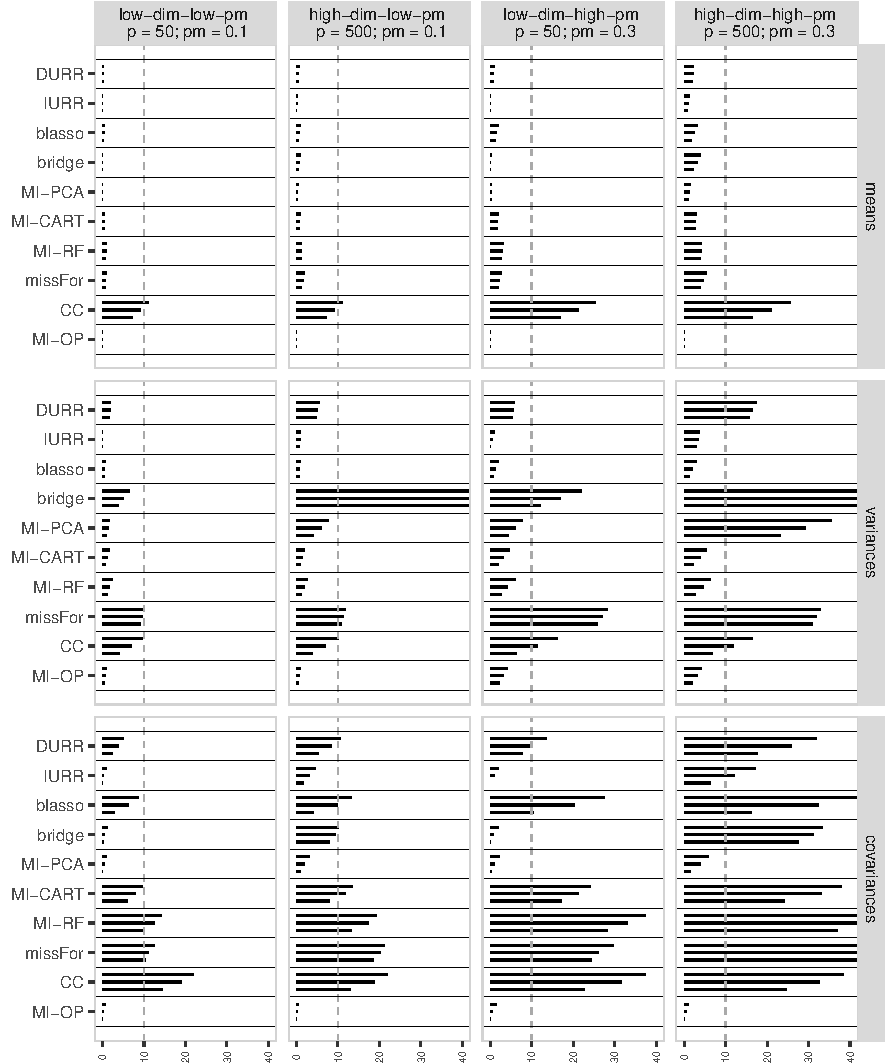
\includegraphics{\pathFIG/exp1_bias_summy.pdf}
\caption{\label{fig:exp1bias}
	Maximum, average, and minimum absolute percent relative bias ($|\text{PRB}|$) for item means, variances, 
	and covariances in Experiment 1.
	}
\end{figure}

\begin{figure}
\centering
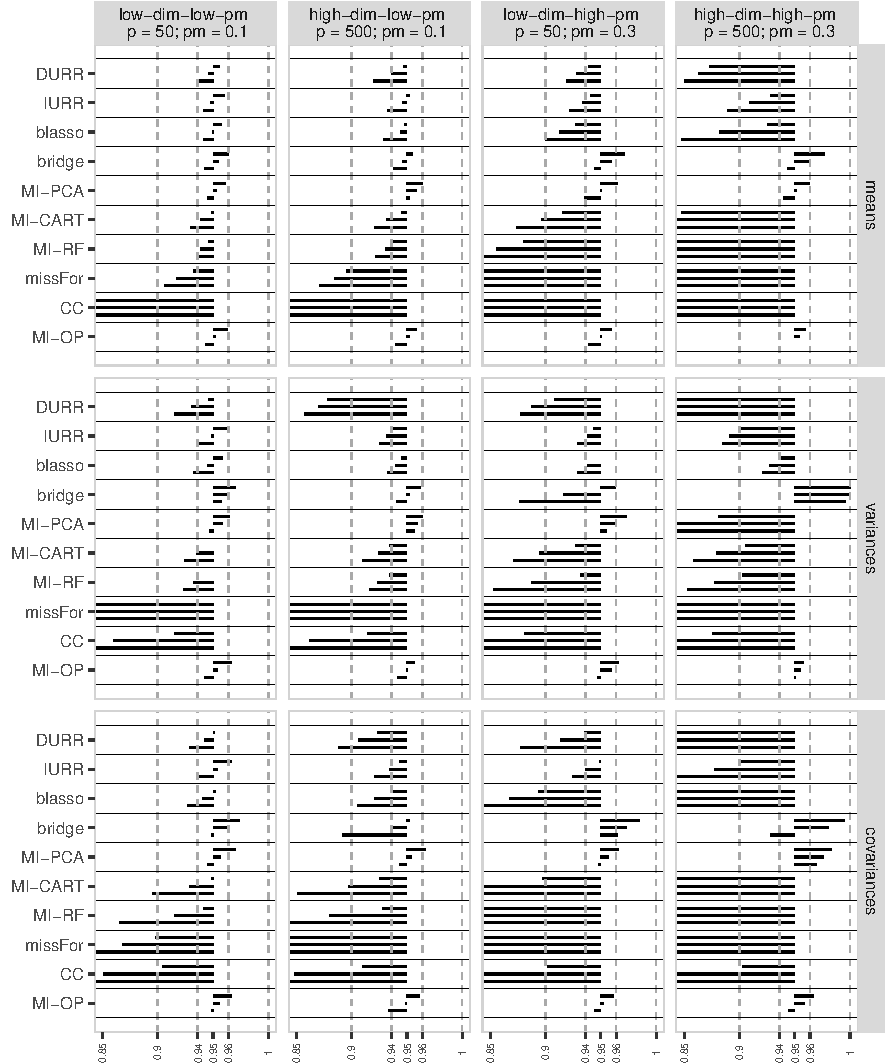
\includegraphics{\pathFIG/exp1_CI_summy.pdf}
\caption{\label{fig:exp1cir}
	Maximum, average, and minimum CIC for item means, variances, and covariances in Experiment 1.
	}
\end{figure}
	
%\FloatBarrier % stops fig:exp1cir to leave its section

